% Proof of the Cut Property; See CLRS (Figure 23.3; 2nd edition)

\documentclass[beamer]{standalone}

\usepackage{tikz}
\usetikzlibrary{calc, shapes, arrows.meta, mindmap, backgrounds, fit}

\begin{document}
\begin{frame}{Proof of the Cut Property}
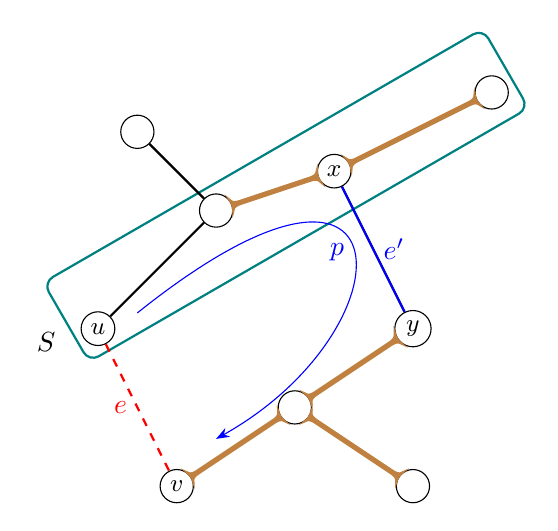
\begin{tikzpicture}[v/.style = {draw, circle, font = \small, inner sep = 2pt, minimum size = 12pt},
		e/.style = {thick},
	mstv/.style = {v, fill = teal},	% vertices in cut property example
	xe/.style = {circle connection bar, thick, brown, fill}, % edges in X
	cut/.style = {rectangle, rounded corners, dashed, draw, thick}	% cut
]
  \uncover<1->{
    \node (v) [v] {$v$};
    \node (v1) [v] at (1.5,1) {};
    \node (v2) [v] at (3,0) {};
  
    \node (y) [v] at (3,2) {$y$};
  
    \node (u) [v] at (-1,2) {$u$};
    \node (u1) [v] at (0.5,3.5) {};
    \node (u2) [v] at (-0.5,4.5) {};
  
    \node (x) [v] at (2,4) {$x$};
    \node (x1) [v] at (4,5) {};
  
    % edges in T
    \draw[e] (v) to (v1) edge (v2) to (y) to (x) edge (x1) to (u1) edge (u2) to (u);
  
    % edges in X
    \draw[xe] (v) to (v1) to (y) (u1) to (x) to (x1) (v1) to (v2);
  }

  % cut
  \uncover<2->{
    \begin{pgfonlayer}{background}
  	  \node<2-> () [draw, thick, rectangle, rounded corners, teal, rotate fit = 30, fit = (u) (u1) (x) (x1), label = {left:$S$}] {};
    \end{pgfonlayer}
  }

  % edge uv
  \uncover<3->{
    \draw[thick, dashed, red] (u) to node[left] {$e$} (v);
  }

  % path uv in T
  \uncover<4->{
    \draw[>=Stealth, ->, blue] ($(u)+(0.5,0.2)$) .. controls ($(x)+(1,1)$) and (y) .. node [left] {$p$} ($(v)+(0.5,0.6)$);
  }

  % path xy in the cut
  \uncover<5->{
    \draw[thick, blue] (x) to node[right] {$e'$} (y);
  }
\end{tikzpicture}
\end{frame}
\end{document}

